\appendix
	\part*{Annexes}	
	\addcontentsline{toc}{part}{Annexes}
	\setcounter{chapter}{0}

\chapter{\label{annexe_index_schoepflin}Les index de la Renaissance, termes contrôlés et classification alphabétique (les index de l'\textit{Alsatia Illustrata} de \nP{Jean-Daniel}{Schoepflin})}
\titreEntete{Annexe \thechapter}

\begin{figure}[!h]
	\centering
	\begin{minipage}[c]{.46\linewidth}
		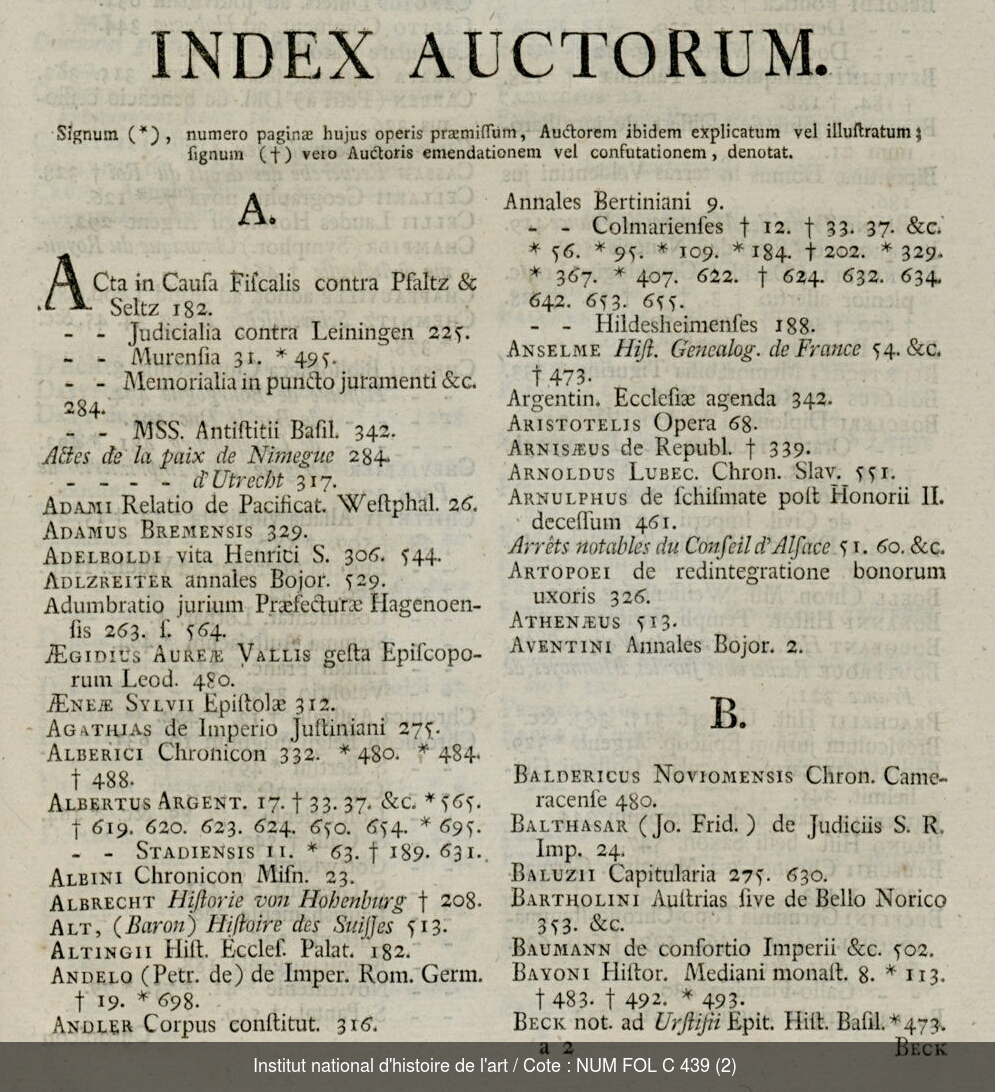
\includegraphics[width=6cm]{images/index_auctorum_alsatia.jpg}
		\caption{Index auctorum}
	\end{minipage} \hfill
	\begin{minipage}[c]{.46\linewidth}
		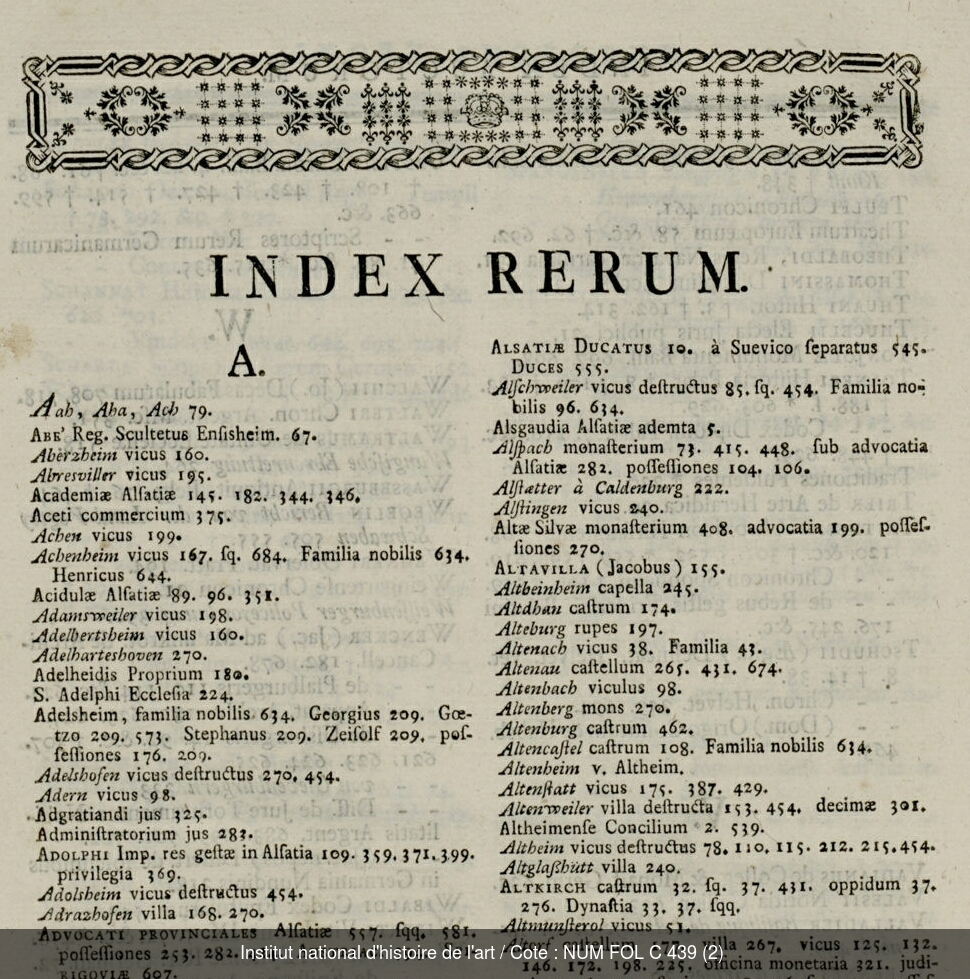
\includegraphics[width=6cm]{images/index_rerum_alsatia.jpg}
		\caption{Index rerum}
	\end{minipage} 
	\medskip
	Extraits des deux index de l'œuvre de \nP{Jean-Daniel}{Schoepflin} [Source: \url{http://bibliotheque-numerique.inha.fr/idurl/1/12532}, p.804 et 813]
\end{figure}

\chapter{\label{annexe_types_interop}Les différents types d'interopérabilité}
\titreEntete{Annexe \thechapter}

\begin{figure}[!h]
	\centering
	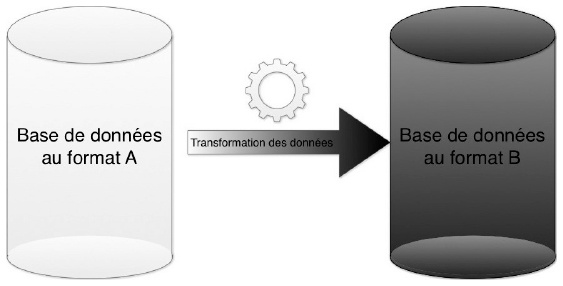
\includegraphics[width=12cm]{images/interop_conversion_copie.jpeg}
	\medskip
	\caption[L'interopérabilité par conversion et copie]{L'interopérabilité par conversion et copie [Source: \cite{bermes_2_2013}]}
\end{figure}

\begin{figure}[!h]
	\centering
	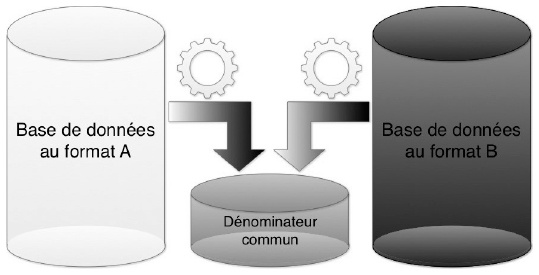
\includegraphics[width=12cm]{images/interop_denom_commun.jpeg}
	\medskip
	\caption[L'interopérabilité par le plus petit dénominateur commun]{L'interopérabilité par le plus petit dénominateur commun [Source: \cite{bermes_2_2013}]}
\end{figure}